\documentclass[12pt]{article}
\usepackage[utf8]{inputenc}
\usepackage[a4paper, margin=2cm]{geometry}
\usepackage{multicol, caption}
\usepackage{authblk}
\usepackage[varg]{txfonts}
\usepackage{titlesec}
%\usepackage[T1]{fontenc}
%\usepackage{lmodern}
% \usepackage[english]{babel}


\usepackage{amsmath}
\usepackage{amssymb}
\usepackage{amsfonts}
\usepackage{graphicx}% Include figure files
\usepackage{dcolumn}% Align table columns on decimal point
\usepackage{bm}% bold math
\usepackage{hyperref}% add hypertext capabilities
\usepackage{minted}
\usepackage[autostyle]{csquotes}

\usepackage[backend=biber,style=numeric]{biblatex}
\addbibresource{bib.bib}

\hyphenpenalty=10000
\exhyphenpenalty=10000

% CUSTOM FORMAT FOR SECTION
\titleformat{\section}[wrap]{\normalfont\bfseries}{\thesection.}{0.5em}{}
\titlespacing{\section}{12pc}{1.5ex plus .1ex minus .2ex}{1pc}
% CUSTOM SUBSECTION
\titleformat{\subsection}[wrap]{\normalfont\bfseries}{\thesubsection.}{0.5em}{}
\titlespacing{\subsection}{12pc}{1.5ex plus .1ex minus .2ex}{1pc}
% CUSTOM SUBSUBSECTION 
\titleformat{\subsubsection}[wrap]{\normalfont\bfseries}{\thesubsubsection.}{0.5em}{}
\titlespacing{\subsubsection}{12pc}{1.5ex plus .1ex minus .2ex}{1pc}

% CUSTOM LINE SPACING (Default 1.2 -> 1.2*1.25=1.5)
\linespread{1.25}

% CUSTOM NAMING
\renewcommand*\contentsname{Summary}

\newenvironment{Figure}
  {\par\medskip\noindent\minipage{\linewidth}}
  {\endminipage\par\medskip}

\title{PHYS6006 Final Report \\
       Magnetospheric structure associated with high-latitude auroras}
\author[1]{J. Plank}
\author[2]{R. C. Fear}
\affil[1, 2]{Department of Physics and Astronomy, University of Southampton}
\date{April 2020}

\begin{document}\sloppy
% TITLE BLOCK
\maketitle

% ABSTRACT
\begin{abstract}
    \noindent\textit{Context:} Only case studies have been done on the magnetospheric structure associated with the formation of high latitude aurora, and the connection of interplanetary magnetic field direction is suspected but has never been quantified.\\
    \textit{Aims:} To produce a statistical survey on the relationship between a northward pointing interplanetary magnetic field and a phenomenon known as transpolar arcs.\\
    \textit{Methods:} Using data from the ESA satellite Cluster, we analysed the ion temperature for many different values of $Z_{GSM}$, covering the plasma sheet as well as the magnetotail lobes.\\
    \textit{Results:} We found a direct link to IMF direction based on high temperature events observed in the lobe, suggesting high-latitude aurora form during periods of northward pointing IMF.
\end{abstract}

\pagebreak

\tableofcontents
\addtocontents{toc}{~\hfill\textbf{Page}\par}
\addtocontents{lof}{~\hfill\textbf{Page}\par}
\bigskip
\listoffigures

\pagebreak

% % SWITCH TO 2 COLUMNS
% \begin{multicols}{2}

\section{INTRODUCTION}
Earth and the Sun are connected by more than just gravity, magnetic interactions between the two bodies are the cause of some of the most dramatic and complex phenomena on Earth. The most well known of these is the aurora (Borealis in the northern hemisphere and Australis in the southern). More commonly known as the northern and southern lights, these light shows come as a result of charged particles flowing along the Sun's magnetic field lines (known as solar wind) and making their way down to Earth in a zone known as the auroral oval \cite{AAAspaceweather}. The Sun's violent nature is also transmitted to Earth along its magnetic field, known as the `Interplanetary magnetic field` (IMF). This can result in satellite damage, radiation hazards to astronauts and airline passengers, telecommunications problems, and outages of power and electronics systems \cite{AAAspaceweather}.

The modern theory of the formation of the aurora was first proposed by Kristian Birkeland in 1903 \cite{birkeland2018norwegian}. He said that auroras are produced when solar wind encounters the geomagnetic field. The result of this is the formation of the plasmasphere in the equatorial plane of Earth's magnetic field \cite{cosmicelectrodyn}.

\subsection{Structure of Earth's magnetic field}
Figure \ref{fig:plasmasphere} is a representation of the solar-terrestrial environment. The solar wind, travelling with the interplanetary magnetic field from the sun \cite{Svalgaard_2010}, is coming from the left. It collides with the terrestrial magnetic field at supersonic speeds, creating a bow shock wave in front of the magnetosphere - the region where magnetic field lines connect to Earth at both ends - the boundary of the magnetosphere is the magnetopause. Supersonic solar winds compress at this boundary creating a magnetosheath between the magnetopause and the bow shock \cite{BSPP}.

\begin{Figure}
    \begin{minipage}[c]{0.57\textwidth}
        \centering
        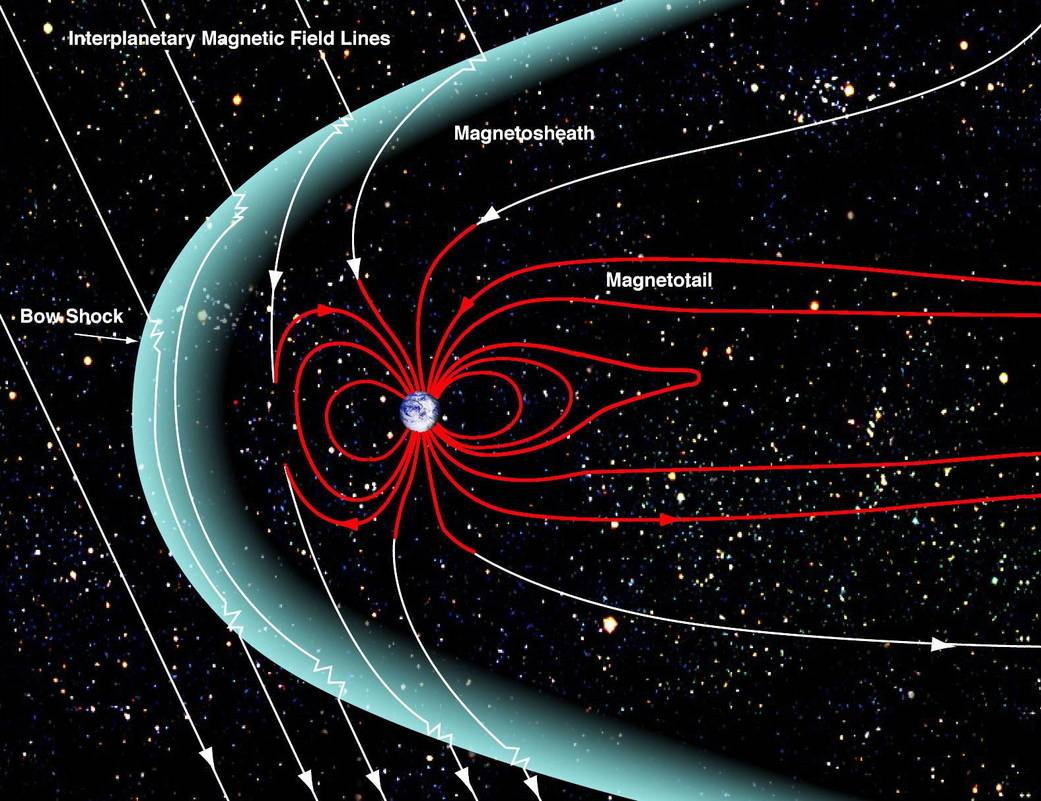
\includegraphics[width=0.7\textwidth]{NASA-Magnetosphere.jpeg}
    \end{minipage}\hfill
    \begin{minipage}[c]{0.4\textwidth}
        \captionof{figure}{Representation of the solar-terrestrial magnetic interaction. The sun is located to the left, producing solar winds and the IMF. Solar winds collide with the terrestrial magnetic field at supersonic speeds, creating a bow shock wave which encases the magnetosphere in a magnetosheath of compressed solar wind \cite{BSPP}. (Image courtesy of NASA)}
        \label{fig:plasmasphere}
    \end{minipage}
\end{Figure}


Write more... 
- Something about GSM coords
- Reconnection

\section{OBSERVATIONS}
The majority of observations in this report come from Cluster, a group of four satellites built by ESA and launched in pairs on Soyuz rockets from Baikonur on the 16th July and 9th August 2000. They fly in a 57hr elliptical polar orbit and are arranged in a tetrahedron formation with a separation of between a few hundred and a few thousand km.

\subsection{Limitations of Cluster's orbit}
The orbit of cluster varies throughout the year. For significant portions of the year the satellite is well outside of the lobes, therefore the best months to extract data are July-October every year, where the spacecraft spends the majority of its time in the tail, and does not enter the magnetosheath. 

Figure \ref{fig:ClusterPos} shows Cluster's orbit through the month of September 2005 as an example, it does not cross the predicted magnetopause boundary (outer dotted parabola). Cluster will also cross through the plasmasphere in every orbit. This leaves the grey shaded region as the area of interest.

\begin{Figure}
    \begin{minipage}[c]{0.57\textwidth}
        \centering
        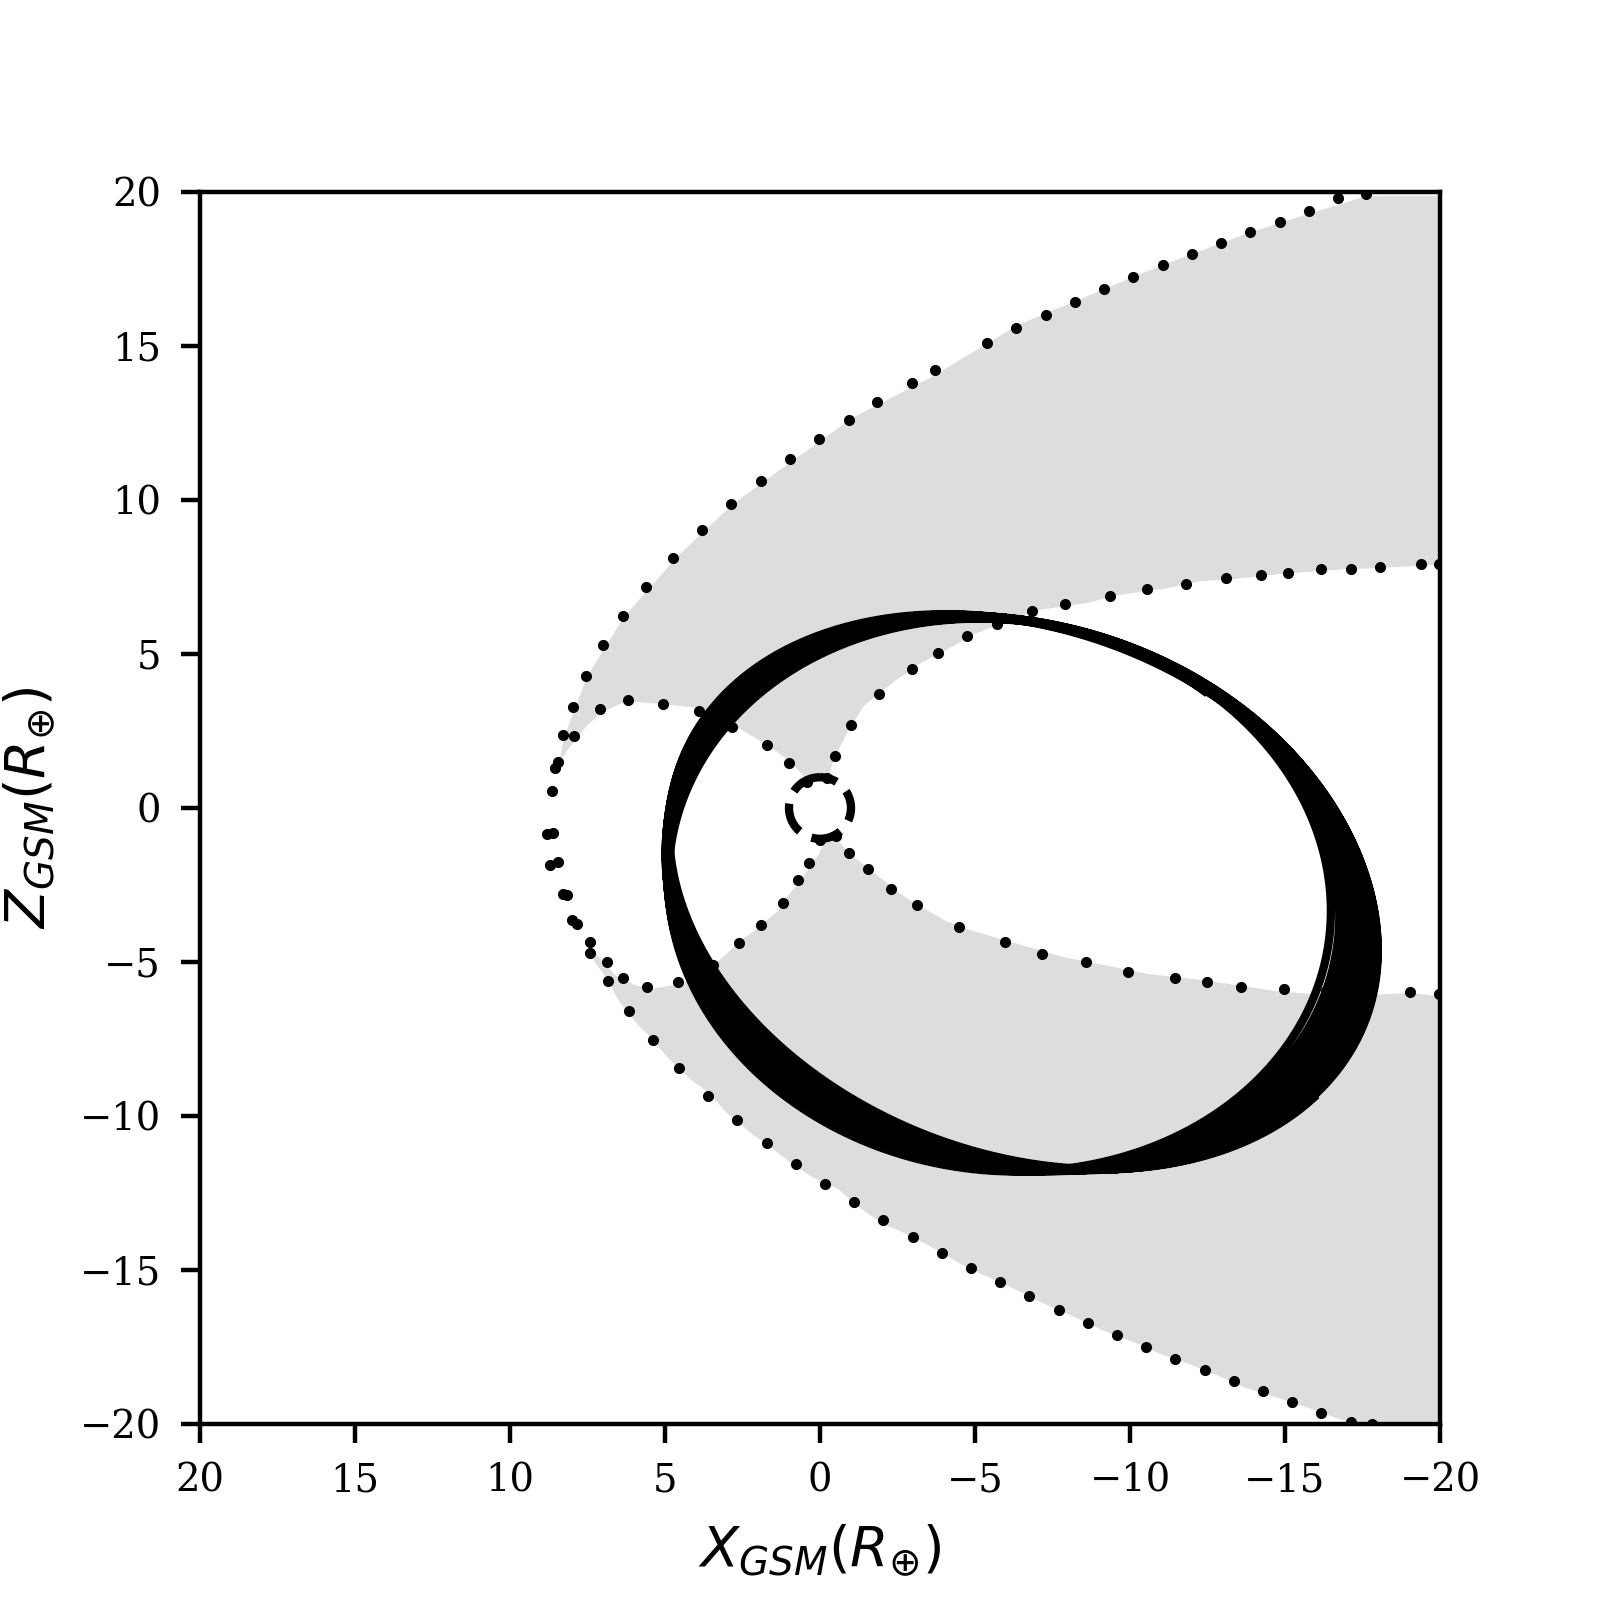
\includegraphics[width=0.7\textwidth]{sc_pos_09_05_coloured.png}
    \end{minipage}\hfill
    \begin{minipage}[c]{0.4\textwidth}
        \captionof{figure}{Plot of Cluster's orbit throughout September 2005 (solid), along with model results for the magnetopause and open-closed boundary on 15/09/2005 (dotted) \cite{Fear1506, substormConfModel}. The grey shaded region is of interest as it contains open field lines. If a reconnection event was detected while the spacecraft was in this region then it could indicate a transpolar arc. Plotting is done in the GSM coordinate system, where +X points to the sun and +Z points along the magnetic dipole axis.}
        \label{fig:ClusterPos}
    \end{minipage}
\end{Figure}

\subsection{High temperatures in the lobe}
Occasionally when Cluster is in the lobe, it will detect periods of uncharacteristically high temperature. There is some debate on the cause of this; Shi \textit{et al} \cite{Shi2013} attribute it to solar wind penetrating into the lobe, whereas Fear \textit{et al} \cite{Fear1506} suggests that this cannot be the case due to the presence of a double loss cone. 

A double loss cone occurs when there is a magnetic mirror at both ends of the field line. This would imply that the observed field line is closed, since the Earth's dipole field has the property where magnetic field strength increases as you travel along a field line to either pole. This would cause an ion to slow down and reverse direction at the poles, i.e. it bounces back and forth from pole to pole.



\subsection{Temperature distribution in the magnetosphere}
Figure \ref{fig:tempLocations} shows the mean distribution of temperatures in the magnetosphere, during the period May to December for years 2002, 2010. We can see the general shape of the plasma sheet, a hot region to the right of the Earth where the normal aurora- generating reconnection happens.

\begin{Figure}
    \begin{minipage}[c]{0.57\textwidth}
        \centering
        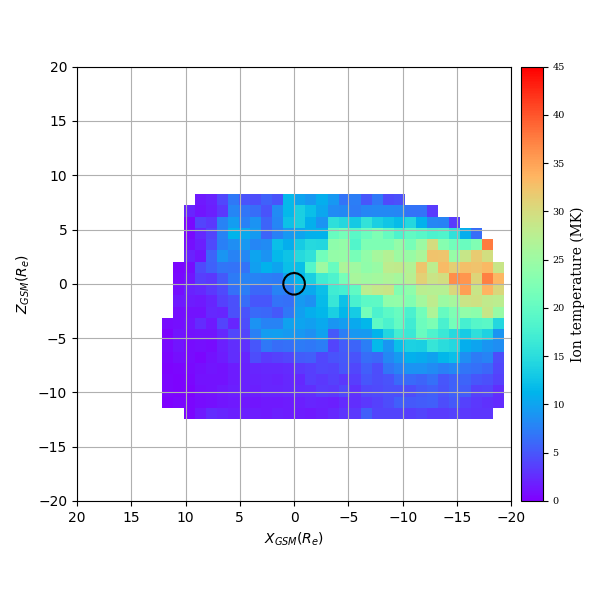
\includegraphics[width=0.9\textwidth]{tempLocations.png}
    \end{minipage}\hfill
    \begin{minipage}[c]{0.4\textwidth}
        \captionof{figure}{The temperature distribution in the magnetosphere. Measurements from Cluster orbits in the months May-December during the years 2002-2010. Each pixel is $1{R_e}^2$ in area, and represents the mean ion temperature when cluster was in that position, blue for lower temperatures and red for hotter. The plasma sheet is visible as a high temperature region to the right of Earth.}
        \label{fig:tempLocations}
    \end{minipage}
\end{Figure}

\subsection{High temperature events}
What constitutes a high temperature? That depends on where in the magnetosphere you are looking. The most easily quantifiable way to separate the plasma sheet from the lobe is to look at the Z coordinate in the Geocentric Solar Magnetospheric (GSM) coordinate system \cite{maus_2006}.

\begin{Figure}
    \begin{minipage}[c]{0.57\textwidth}
        \centering
        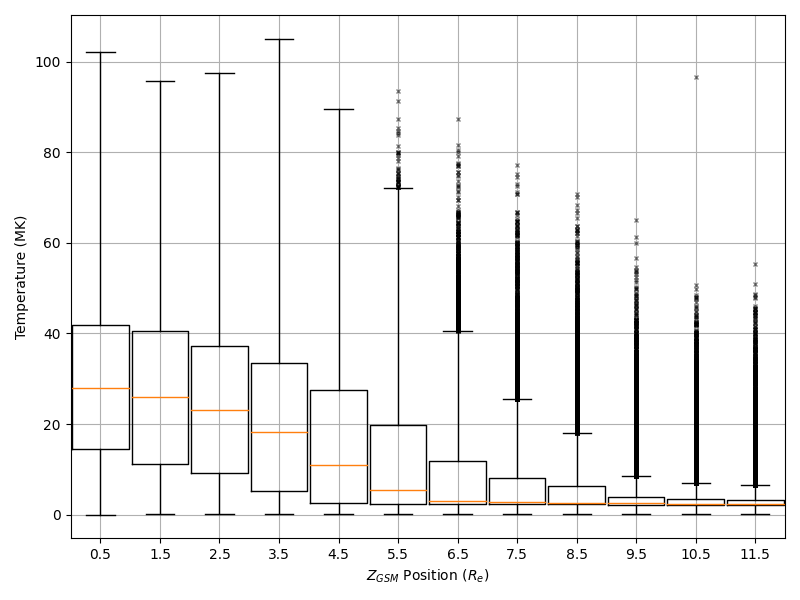
\includegraphics[width=\textwidth]{avg_temp_z.png}
    \end{minipage}\hfill
    \begin{minipage}[c]{0.4\textwidth}
        \captionof{figure}{Box plot of the temperature distribution as a function of $Z_{GSM}$. Each box covers a width of $1R_e$, starting at $[0,1)$ $R_e$ then $[1,2)$ $R_e$ etc until $[11,12]$ $R_e$. Yellow lines represent the median, each box is the interquartile range of each bin, and the ``whiskers'' are maximum and minimum values, up to $3\times IQR$. Outliers plotted as black `$\times$'. The box centred at $5.5R_e$ (for the interval $[5,6)$ $R_e$) suggests that temperatures above $\approx20MK$ are good candidates for high temperature events. Data is from Jul-Oct 2002-2010 for $X_{GSM}<0$ $R_e$.}
        \label{fig:avg_temp_z}
    \end{minipage}
\end{Figure}

We can see from Figure \ref{fig:tempLocations} that the plasma sheet ends at approximately $Z_{GSM}=\pm6R_e$. Giving an exact position for the edge of the plasma sheet is difficult as it is dynamic and in this project we were using measurements from many months and years.

In figure \ref{fig:avg_temp_z} we created a box plot of measurements from July-October 2002-2010 (for $X_{GSM} < 0$, i.e. excluding points sunwards of Earth). Taking the estimation from above that the plasma sheet ends at $\approx6R_e$, we can see from the box centred on $5.5R_e$ that temperatures exceeding $\approx 20MK$ can reasonably be considered uncharacteristically high.

\subsection{Duration of events}
The event analysed by Fear \textit{et al} \cite{Fear1506} on 15-09-2005 lasted for approximately 2 hours. In figure \ref{fig:aur_comp} we analyse the length of each of our events detected in the same time period as above (Jul-Oct 2002-2010), plotting the result as a histogram. Repeating this for various cutoff points based on $|Z_{GSM}|$ gives a view of how the length of each event changes over time. 

\begin{Figure}
    \centering
    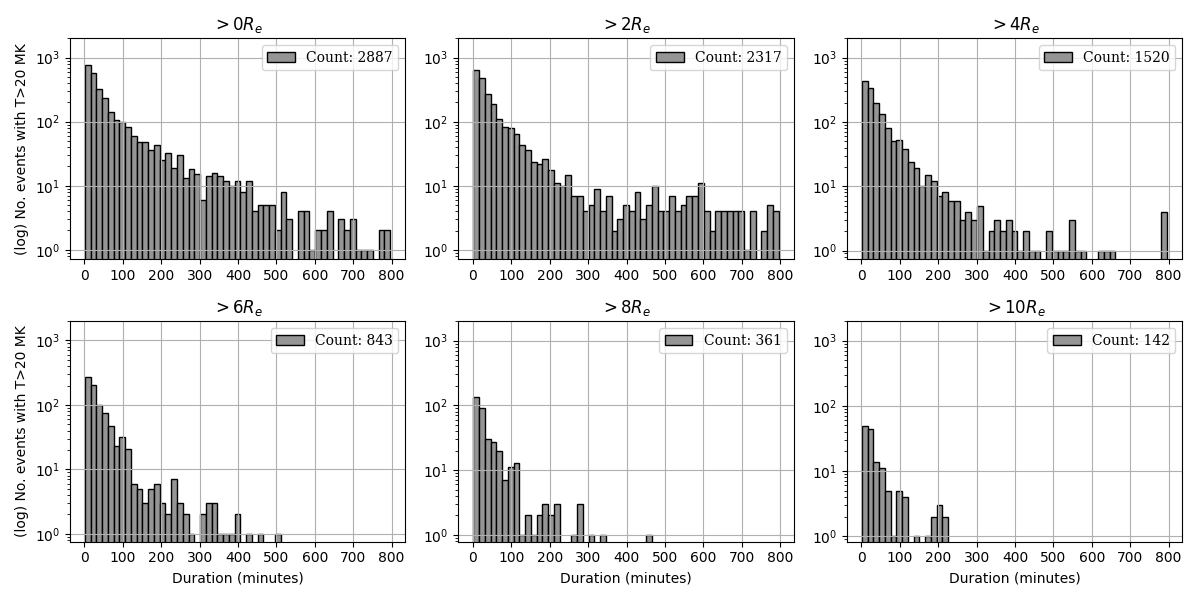
\includegraphics[width=\textwidth]{aur_comp.png}
    \captionof{figure}{Histograms showing the number of events with a certain duration (in minutes). Each panel shows a different cutoff point for $|Z_{GSM}|$. Very long duration events are consistent with passing through the plasma sheet where having a temperature above $20MK$ for over 10 hours is possible. Therefore as the $Z$ cutoff is increased we would expect those long duration events to become less common as measurements outside of the plasma sheet are excluded. What is left is $732$ (see $>6 R_e$ panel) high temperature events occurring outside the region where they are expected.}
    \label{fig:aur_comp}
\end{Figure}

We see that when the plasma sheet is excluded by excluding results where $|Z_{GSM}|<6R_e$, there are $732$ events left. This works out to be just under one per day ($732/984\approx0.75\ events/day$). The properties of this distribution are shown in table \ref{tab:event_durn}. This shows that these events are comparable in length to the 15-09-2005 event.

Many short duration events are likely to be noise. Although cluster makes a full rotation approximately every three seconds and can therefore provide measurements with similar resolution, the choice was made to average the data into five minute bins, which would match with the predicted geometric position data from \cite{cdms}, and the IMF components parameters obtained from NASA/GSFC's OMNI data set through OMNIWeb \cite{omniData}.

\begin{table}[]
    \begin{minipage}[c]{0.57\textwidth}
        \centering
        \begin{tabular}{||c|l||c|l||}
            \hline
            count & 732 & $25\%$ & 00:15:00 \\
            mean & 01:16:18 & $50\%$ & 00:25:00 \\
            std & 03:38:36 & $75\%$ & 01:00:00 \\
            min & 00:10:00 & max & 1 day 12:40:00 \\
            \hline
        \end{tabular}
    \end{minipage}\hfill
    \begin{minipage}[c]{0.4\textwidth}
        \caption{Statistical properties for the duration of events occurring at $|Z_{GSM}|>6R_e$.}
        \label{tab:event_durn}
    \end{minipage}
\end{table}

\subsection{The Interplanetary Magnetic Field}
The IMF data consists of three measurements from OMNI, $B_x, B_y, B_z$, all in the GSM coordinate system. 

\section{RESULTS}

\section{DISCUSSION}
HI

\section{CONCLUSION: FUTURE WORK}
HI \\

\printbibliography
% \end{multicols}
\end{document}